\documentclass[12pt, twoside]{article}
\usepackage[francais]{babel}
\usepackage[T1]{fontenc}
\usepackage[latin1]{inputenc}
\usepackage[left=1cm, right=1cm, top=7mm, bottom=7mm]{geometry}
\usepackage{float}
\usepackage{graphicx}
\usepackage{array}
\usepackage{multirow}
\usepackage{amsmath,amssymb,mathrsfs}
\usepackage{soul}
\usepackage{textcomp}
\usepackage{eurosym}
 \usepackage{variations}
\usepackage{tabvar}

\pagestyle{empty}
\begin{document}

\begin{center}
\fbox{Correction du contr�le 1}
\end{center}

\ul{Exerices 5 et 6}:

\enskip

\fbox{
\begin{minipage}{18cm}
C'est la derni�re op�ration � effectuer qui d�termine le nom de
l'expression (le premier mot de la phrase ).
\end{minipage}
}


\enskip

La diff�rence du produit de -3 par -2 et de 1: $(-3) \times (-2) -1$

Le quotient de la somme de 6 et -7 par le produit de 1 par -2:
$\dfrac{6+(-7)}{1 \times (-2)}$ ou  $\big( 6+(-7) \big) \div \big( 1 \times
(-2) \big)$


\enskip

$(-5)+3 \times (-4)$ $\to$ La somme de (-5) et du produit de 3 par (-4)

$(-8-3) \times (-2)$ $\to$ Le produit de la diff�rence de -8 et de 3 par -2. 



\bigskip

\bigskip


\ul{Exercice 3}: Compl�ter les phrases suivantes:

$\bullet$ Le produit de deux nombres relatifs de m�me signe est \ldots \ldots \ldots

$\bullet$ Le produit de deux nombres relatifs de signes contraires est \ldots
\ldots \ldots


\enskip

En s'aidant du sch�ma ci-dessous, d�terminer le signe des produits suivants:

Exemple: 

\begin{center}
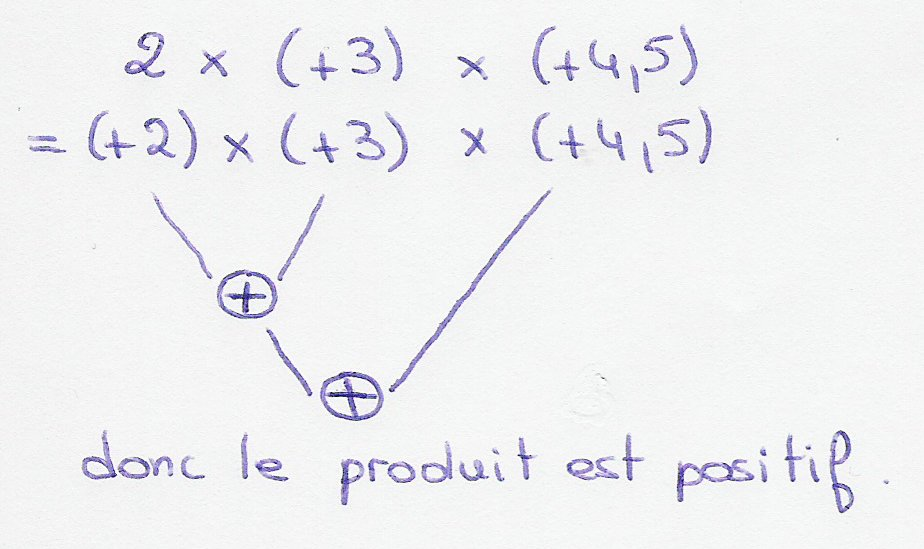
\includegraphics[width=6cm]{images/ex1.jpg}
\end{center}

A compl�ter:

\begin{center}
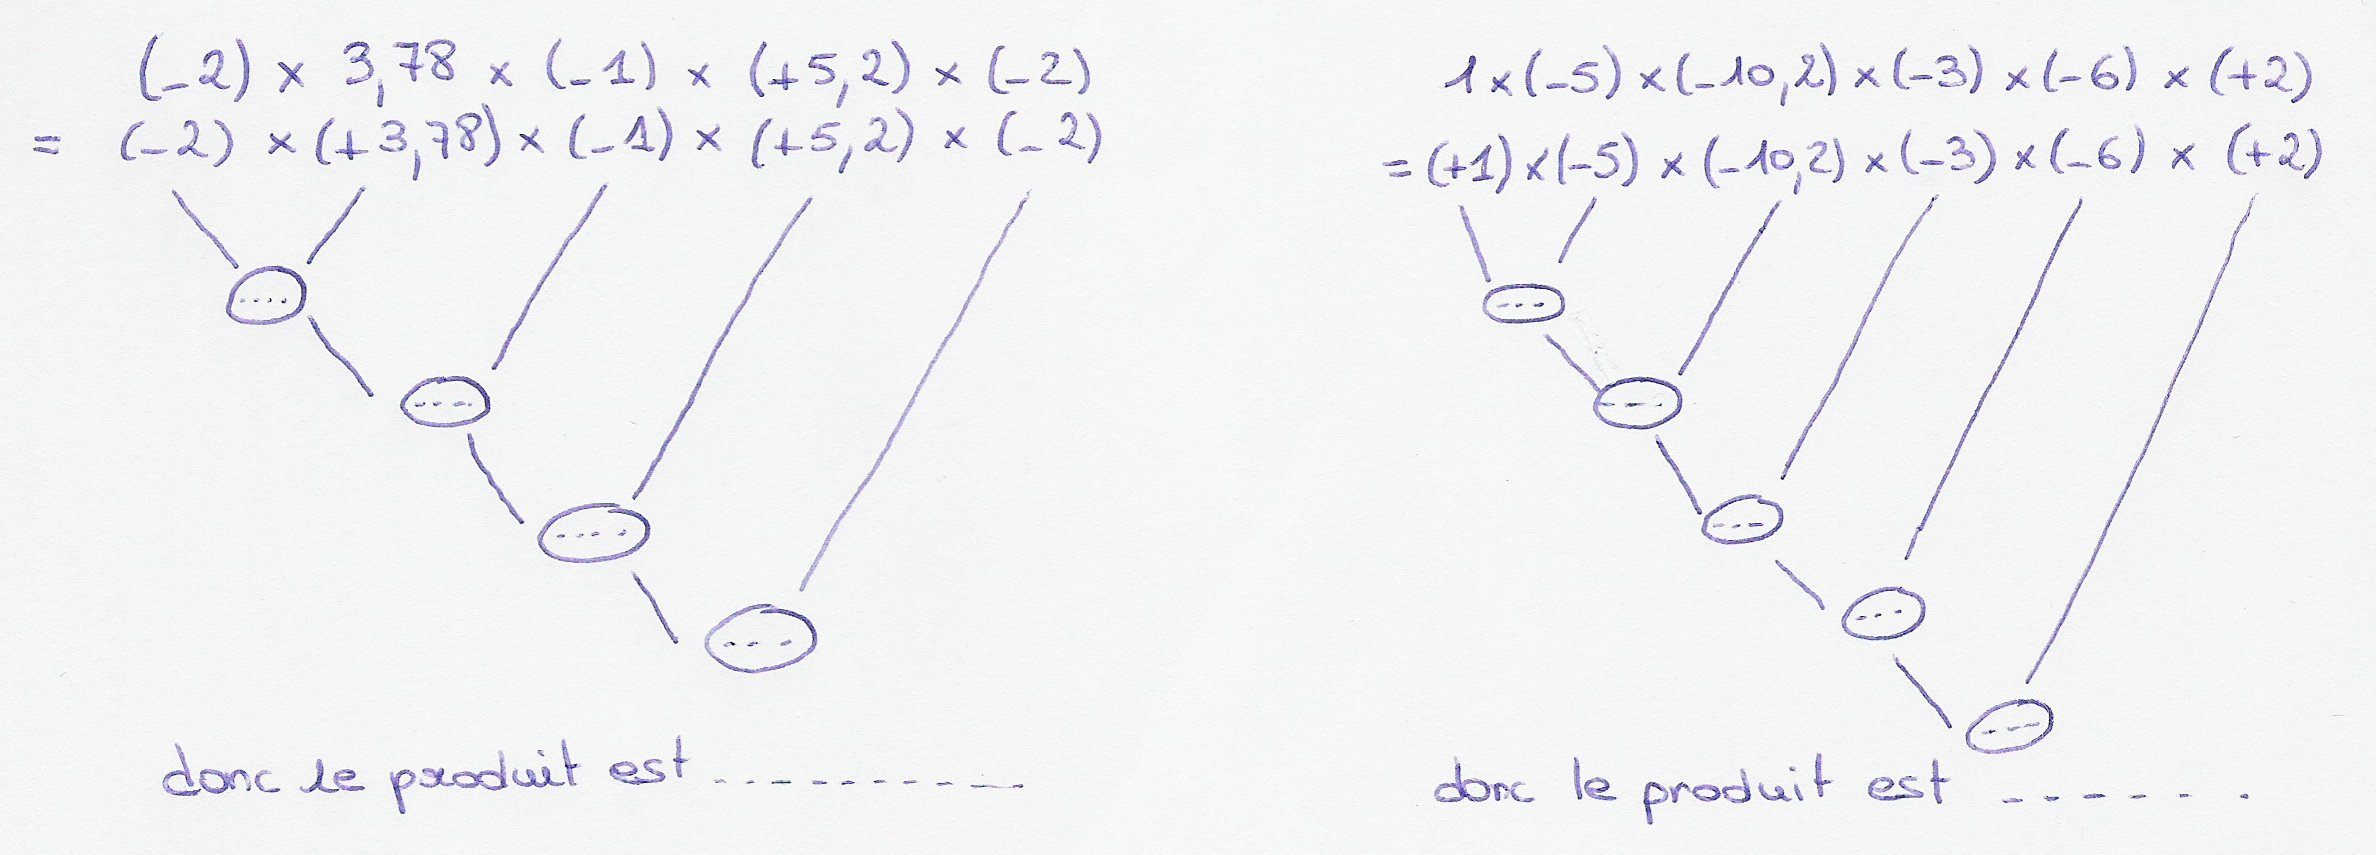
\includegraphics[width=17cm]{images/ex2.jpg}
\end{center}


\bigskip


\ul{Exercice 4}:


\begin{tabular}{ccc}
$A=-2-3 \times (+4)$ & $\leftarrow$ & 
\begin{minipage}{13cm}
je commence par \ldots \ldots \ldots
\ldots \ldots \ldots \ldots \ldots

\enskip

\end{minipage} \\


\medskip

\medskip

$=-2- $\ldots \ldots  \ldots & $\leftarrow$ & 
\begin{minipage}{13cm}
le produit de deux nombres relatifs de m�me signe est \ldots \ldots \ldots
\ldots \ldots et je \ldots \ldots \ldots \ldots \ldots \ldots \ldots les
distances � z�ro \end{minipage} \\

\medskip

\medskip

 $=(-2) + $\ldots \ldots & $\leftarrow$ &
\begin{minipage}{13cm}
pour soustraire deux nombres relatifs, on \ldots \ldots \ldots \ldots  \ldots
\ldots 
\end{minipage} \\


\medskip

\medskip

$=$ \ldots \ldots \ldots & $\leftarrow$ & 
\begin{minipage}{13cm}
pour additionner deux nombres relatifs de m�me signe:

1) choix du signe: \ldots \ldots \ldots \ldots \ldots \ldots \ldots \ldots
\ldots \ldots \ldots

2) \ldots \ldots \ldots \ldots \ldots \ldots \ldots \ldots \ldots \ldots les
distances � z�ro
\end{minipage}

\end{tabular}
 
\bigskip





\begin{tabular}{ccc}
$B= 3 \times 6 -2 \times 7 -6$ & $\leftarrow$ &
\begin{minipage}{13cm}
je commence par les \ldots \ldots \ldots
\ldots \ldots \ldots \ldots \ldots

\enskip

\end{minipage} \\

$= \ldots - \ldots  -6$  \quad \quad &  & \\

\medskip

\medskip

$=4-6$ \qquad \qquad \qquad & $\leftarrow$ &
\begin{minipage}{13cm}
dans une suite d'additions et de soustractions, j'effectue les
calculs \ldots \ldots \ldots \ldots \ldots \ldots \ldots
\end{minipage} \\

\medskip

\medskip

$=4 + (\ldots \ldots$) \quad \qquad & $\leftarrow$ &
\begin{minipage}{13cm}
pour soustraire deux nombres relatifs, on \ldots \ldots \ldots \ldots  \ldots
\ldots 
\end{minipage} \\

\medskip

\medskip

$=\ldots \ldots \ldots$ \qquad \qquad  &   $\leftarrow$       &
\begin{minipage}{13cm}
pour additionner deux nombres relatifs de signes contraires:

1) choix du signe: \ldots \ldots \ldots \ldots \ldots \ldots \ldots \ldots
\ldots \ldots \ldots

2) \ldots \ldots \ldots \ldots \ldots \ldots \ldots \ldots \ldots \ldots les
distances � z�ro
\end{minipage}

\end{tabular}


\bigskip


\bigskip


\bigskip


\bigskip



\begin{tabular}{ccc}
$C= 4 \times (-6+8) -12$ & $\leftarrow$ &
\begin{minipage}{13cm}
je commence par \ldots \ldots \ldots
\ldots \ldots \ldots \ldots \ldots

\enskip

\end{minipage}\\

$=4 \times (\ldots \ldots )-12$  & $\leftarrow$ &
\begin{minipage}{13cm}
pour additionner deux nombres relatifs de signes contraires:

1) choix du signe: \ldots \ldots \ldots \ldots \ldots \ldots \ldots \ldots
\ldots \ldots \ldots

2) \ldots \ldots \ldots \ldots \ldots \ldots \ldots \ldots \ldots \ldots les
distances � z�ro

\bigskip


\end{minipage} \\

\medskip

\medskip



$=(\ldots \ldots) -12$ \qquad \quad & $\leftarrow$ &
\begin{minipage}{13cm}
je commence par \ldots \ldots \ldots
\ldots \ldots \ldots \ldots \ldots

\enskip

\end{minipage}\\

$=8+ (\ldots \ldots)$ \qquad \qquad & $\leftarrow$ &
\begin{minipage}{13cm}
pour soustraire deux nombres relatifs, on \ldots \ldots \ldots \ldots  \ldots
\ldots 

\bigskip


\end{minipage} \\

\medskip

\medskip

$= \ldots \ldots$ \qquad \qquad & $\leftarrow$ &
\begin{minipage}{13cm}
pour additionner deux nombres relatifs de signes contraires:

1) choix du signe: \ldots \ldots \ldots \ldots \ldots \ldots \ldots \ldots
\ldots \ldots \ldots

2) \ldots \ldots \ldots \ldots \ldots \ldots \ldots \ldots \ldots \ldots les
distances � z�ro
\end{minipage} 
\end{tabular}


\bigskip


\bigskip

\bigskip


\bigskip

Pour calculer D: on doit calculer le num�rateur et le d�nominateur (en
respectant les priorit�s et les r�gles de calculs) puis on effectue la division.

$D=\dfrac{2-7 \times (-5)+8}{-5-1+(-3) \times (-5)}$

\bigskip


\quad $= \dfrac{2-(-35)+8}{-5-1+(+15)}$

\bigskip

\quad $=\dfrac{2+35+8}{(-5)+(-1)+15}$

\bigskip

\quad $=\dfrac{45}{9}$

\bigskip

\quad $=5$

\end{document}
